\chapter{ОБЗОР ЛИТЕРАТУРЫ}\label{chap1}
В настоящей глава формулируются основные понятия и определения, используемые в курсовой работе. Приводится классификация (согласно работе \cite{GabasovKirillovaPU}) принципов управления, используемых в современной теории управления. Объясняется принцип управления в режиме реального времени в применении к реализации оптимальных обратных связей в задачах оптимального управления с конечным горизонтом планирования \cite{GabasovDmitrukKirillova15a}.


%%%%%%%%%%%%%%%%%%%%%%%%%%%%%%%%%%%%%%%%%%%%%%%%%%%%%%%%%%%%%%%%%%%%%%%%%%%%%%%%
\section{Задачи оптимального управления}\label{1sec:optimal-control}
Человек занимается управлением на протяжении всей своей жизни для обеспечения желаемого течения тех или иных процессов или сам предпринимает необходимые действия и принимает соответсвующее решения.

Теория оптимального управления, отражающая современный этап развития вариационного исчилсения, возникла в середине \RNumb{20} века в связи с задачами, поставленными практикой в различных областях развития новой техники.

Существует два взгляда на теорию оптимального управления. Согласно одному из них, теория оптимального управления — раздел современного вариационного исчисления. В соответствии с этим взглядом дадим следующее определние.
Управления — элементы функциональных пространств, по которым ищется экстремум выбранного функционала качества. Главной задачей данной теории является анализ решения экстремальной задачи (существование, единственность, непрерывная зависимость решений, необходимые и достаточные условия оптимальности).

Другой взгяд трактует данную теорию как раздел современной теории управления, представляющей естественное развитие классической теории управления. В этом случае выделим следующее определения для управления. Управления — это процесс, в котором для достижения нужного поведения объекта управления в каждый текущий момент времени создаются целенаправленные (управляющие) воздействия на объект управления в зависимотси от доступной к этому моменту информации о поведении объекта и действующих на него возмущений.

%%%%%%%%%%%%%%%%%%%%%%%%%%%%%%%%%%%%%%%%%%%%%%%%%%%%%%%%%%%%%%%%%%%%%%%%%%%%%%%%
\section{Программные и позиционные решения}\label{1sec:Solution}

При управлении динамическим объектом используются три принципа: управление по разомкнутому контуру (программное управление), управление по замкнутому контуру (позиционное управление), управление в реальном времени.

\begin{figure}[h]

\centering

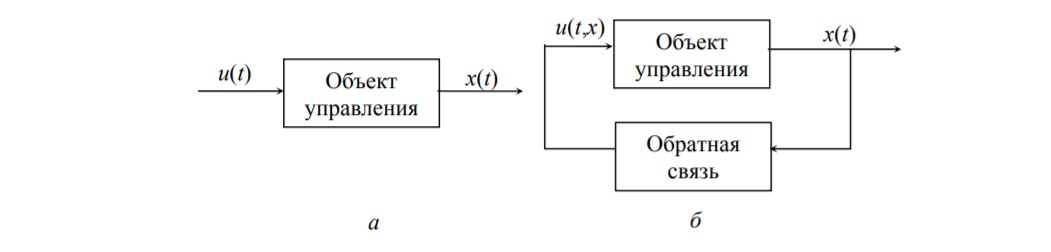
\includegraphics[width=\linewidth]{image1.jpg}

\caption{а) разомкнутый контур; б) замкнутый контур}

\label{fig:mpr}

\end{figure}

\begin{definition} 
Программное управление — управление, при котором (программные) управляющие воздействия (программы) планируются по априорной информации до начала процесса управления и не корректируются в процессе управления. 
\end{definition}

Программное управление редко применяется на практике, поскольку не учитывает неточности математического моделирования физических систем и возмущения, косвенная информация о которых доступна, как правило, в процессе управления. Фундаметом этого метода является принцип максимума Понтрягина. 

\begin{definition} 
Позиционное управление — управление, при котором (позиционные) управляющие воздействия создаются в процессе управления по текущим позициям, которые аккумулируют информацию, доступную к текущему моменту.
\end{definition}

%Динамическое программиирование является одним из основных методов реализации позиционного управления.

\begin{definition} 
Cинтез оптимальных систем управления — построение оптимальных позиционных управляющих воздействий.
\end{definition}
При создании систем по принципу замкнутого контура используются связи трех типов:\emph{прямые}, \emph{обратные} и \emph{комбинированные} (рис. 1.2).
\begin{figure}[h]

\centering

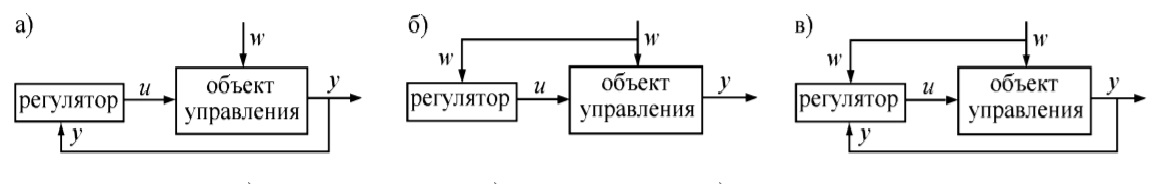
\includegraphics[width=\linewidth]{image2.jpg}

\caption{а) обратная связь; б) прямая связь; в) комбинированная связь}

\label{fig:mpr}

\end{figure}

 Связь называется прямой, если она преобразует в управляющее воздействие доступную информацию о наблюдаемых входных сигналах. Обратная связь по состоянию преобразует в управляющее воздействие информацию о состоянии объекта. В комбинированной связи преобразуется информация обоих типов.
 
 Для позиционного управления характерна следующая особенность. Проблема синтеза в рамках принципа управления по замкнутому контуру не удается решить из-за проклятия размерности ни с помощью принципа максимума, ни с помощью динамического программирования Беллмана. 
 
 Решение данной проблемы состоит в переходе к современному принципу управления — оптимальному управлению в реальном времени. При управлении динамическим объектом в реальном времени связи не строятся, а необходимые для управления их текущие значения формируются в реальном времени по ходу каждого конкретного процесса.
 


%%%%%%%%%%%%%%%%%%%%%%%%%%%%%%%%%%%%%%%%%%%%%%%%%%%%%%%%%%%%%%%%%%%%%%%%%%%%%%%%

\section{Реализация оптимальных обратных связей в реальном времени}\label{1sec:Feedback}
Принцип управления в реальном времени и подход к реализации оптимоной обратной связи в реальном времени опишем на примере следующей задачи оптимального управления.

\begin{equation} \label{1problem}
    c^Tx(t_f)\to \min,
    \end{equation}
$$
    \dot{x}=A(t)x+B(t)u,\quad x(t_0)=x_0^*,
    $$
$$
    x(t_f) \in X_f,\quad  u(t)\in U, \quad  t\in T = [t_*, t^*],
    $$
где  $x = x(t)\in \mathbb{R}^n$ — состояение модели управления в момент времени $t$,
$u = u(t)\in \mathbb{R}^r$ — значение управляющего воздействия в момент $t$, 
$A(t)\in \mathbb{R}^{n\times n}$,
$B(t)\in \mathbb{R}^{n\times r}$,
$x_0^*$ — известное начальное состояние объекта.
$X_f=\{x\in \mathbb{R}^n: g_*\leq Hx \leq g^*\}$ --- терминальное
множество, $H\in \mathbb{R}^{m\times n}$, $g_*,$ $g^* \in \mathbb{R}^m$;
$U=\{u\in \mathbb{R}^r: u_*\le u\le u^*\}$ --- множество доступных значений
управляющего воздействия.

\begin{definition}  Управляющее воздействие $u(t)\in U$, $t\in T$, называется программой, если соответствующая ему
траектория $x(t)$, $t\in T$, математической модели (\ref{1problem}) удовлетворяет
условию $x(t_f)\in X_f$.
\end{definition}

\begin{definition}  Программа $u^0(t)$, $t\in T$,
называется оптимальной (программным решением задачи (\ref{1problem})), если на соответствующей ей (оптимальной) траектории $x^0(t)$, $t\in T$, выполняется равенство $c^Tx^0(t_f) = \min_u c^Tx(t_f),$ где минимум ищется среди всех программ. 
\end{definition}
%%%%%%%%%%%%%%%%%%%%%%%%%%%%%%%%%%%%%%%%%%%%%%%%%%%%%%%%%%%%%%%%%%%%%%%%%%%%%%%%

Задача (\ref{1problem}) рассматривается в классе дискретных управляющих воздействий:

$u\equiv u(\tau), t\in [ \tau,\tau + h[, \tau = T_h = \{t_*,t_* + h,...,t^* - h\} (h = (t^* - t_*)/N, N > 0)$.

Чтобы ввести понятие классической оптимальной обратной связи, погрузим задачу (\ref{1problem}) в семейство задач

\begin{equation} \label{2problem}
    c^Tx(t_f)\to \min,
    \end{equation}
$$
    \dot{x}=A(t)x+B(t)u,\quad  x(\tau) = z,
    $$
$$
    x(t_f) \in X_f,\quad  u(t)\in U, \quad  t\in T(\tau) = [\tau, t^*],
    $$
    
Пусть $u^0(t|\tau,z),\quad t\in T(\tau),$ — оптимальная программа задачи (\ref{2problem})) для позиции ($\tau$,z).

Функция
\begin{equation} \label{3problem}
    u^0(\tau,z) = u^0(\tau|\tau,z),\quad z\in X_\tau,\quad \tau \in T_h,
    \end{equation}
называется оптимальной обратной связью (позиционным решением задачи (\ref{1problem})).

Оптимальная обратная связь (\ref{3problem}) предназначена для управления физическим объектом. Замкнем ею объект управления и запишем поведение замкнутой системы в форме
\begin{equation} \label{4problem}
\dot{x}=A(t)x+B(t)u^0(t,x) + \omega,\ x(t_*) = x_0,
 \end{equation}
где $u^0(t,x) = u^0(t,x(t)) \equiv u^0(\tau,x(\tau)),\quad t\in [\tau,\tau + h[,\quad \tau\in T_h$, $\omega$ — возмущение, действующее на физичиский объект в процессе управления.
\\
Рассмотрим поведение систымы (\ref{4problem}) в конкретном процессе управления.
$$\dot{x^*(t)}=A(t)x^*(t)+B(t)u^0(t,x^*(t)) + \omega^*(t),\quad x^*(t_*) = x_0,$$
$$u^*(t)\equiv u^0(\tau,x^*(\tau)) = u^0(\tau|\tau,x^*(\tau)),\quad t\in[\tau,\tau + h[,\quad  \tau \in T_h,$$

Функцию $u^*(t), t\in T$, будем называть реализацие опитмальной обратной связи (\ref{3problem}) в конкретном процессе управления. 


Перейдём к описанию принципа оптимального управления в реальном времени, при котором обратная связь  (\ref{3problem}) не строится, а при каждом $\tau \in T_h$ текущее управляющее воздействие $u^*(\tau)$ создаётся в процессе управления для текущей позиции $(\tau,x^*(\tau))$.

Пусть  $\delta(\tau)$ — время вычисления значения $u^*(\tau), \tau \in T_h$.
\begin{definition}
Устройство, способное вычислять значение $u^*(\tau), \tau \in T_h$ за время $\delta(\tau) < h$, называется оптимальным регулятором, реализующим оптимальную обратную связь (\ref{3problem}) в реальном времени.
\end{definition}

Из определия оптимальной обратной связи, оптимальный регулятор в каждый момент времени $\tau \in T_h$ должен решить задачу

\begin{equation} \label{5problem}
    c^Tx(t_f)\to \min,
    \end{equation}
$$
    \dot{x}=A(t)x+B(t)u,\quad x(\tau) = x^*(\tau),
    $$
$$
    x(t_f) \in X_f,\quad  u(t)\in U, \quad  t\in T(\tau).
    $$
\\
Для решения задачи (\ref{5problem}) будем использовать динамическую реализацию специального двойственного метода линейного программирования, исходя из следующих особенностей задачи, стоящей перед оптимальным регулятором. 
\\
Предположим, что оптимальный регулятор в предыдущий момент $\tau - h$ для вычисления значения $u^*(\tau - h)$ решил задачу (\ref{2problem}) для позиции $(\tau - h, x^*(\tau - h))$:
\begin{equation} \label{6problem}
    c^Tx(t_f)\to \min,
    \end{equation}
$$
    \dot{x}=A(t)x+B(t)u,\quad  x(\tau - h) = x^*(\tau - h),
    $$
$$
    x(t_f) \in X_f,\quad  u(t)\in U, \quad  t\in T(\tau - h).
    $$
\\    
Управляющее воздействие $u^*(t)\equiv u^0(\tau - h|\tau - h, x^*(\tau - h)), t\in[\tau - h,\tau [,$ поданное на физический объект управления,вместе с возмущение $\omega^*(t)$, $t\in [\tau - h, \tau[$, перевод его в состояние $x^*(\tau)$. 
При малых периодах квантования h и ограниченных возмущениях $\omega(t), t \in T $, это состояние незначительно отличается от состояния $x^0(\tau)$, в которое перешел бы объект управления (\ref{4problem}) при отсутствии возмущения.
Таким образом, можно говорить о малом отличии (в смысле близости точек переключения оптимальных программ) задачи (\ref{6problem}) решённой оптимальным регулятором на промежутке $[\tau - h, \tau[$, от задачи (\ref{5problem}), которую он должен решить на промежутке $[\tau, \tau + h[$.
Поскольку при вычислении оптимальных программ основные затраты времени падают на интегрирование дифференциальных уравнений, то предложенный двойственный метод решения задачи (\ref{5problem}) быстро находит точки переключения новой оптимальной программы $u^0(t| \tau, x^*(\tau)), t\in T(\tau)$, используя информацию о точках переключения оптимальной программы $u^0(t|\tau - h, x^*(\tau - h)), t \in T(\tau - h)$. 
Можно сделать вывод, что текущие значения оптимальной обратной связи можно эффективно вычислять с помощью двойственного метода линейного программирования.

В настоящей глава были рассмотрены основные понятия и определения. Была описана классификация принципов управления, используемых в современной теории управления. Рассмотрен принцип управления в режиме реального времени в применении к реализации оптимальных обратных связей в задачах оптимального управления с конечным горизонтом планирования.
\bigskip